\documentclass[tikz,border=8pt]{standalone}
% Shared look for every TikZ diagram. Load with \input{../../tools/tikz-style.tex}
\usepackage[sfdefault]{roboto}
\usetikzlibrary{arrows.meta, positioning, shapes.geometric, calc, fit, backgrounds}
\definecolor{cblue}{HTML}{4C78A8}
\definecolor{corange}{HTML}{F58518}
\definecolor{cgreen}{HTML}{54A24B}
\definecolor{cred}{HTML}{E45756}
\definecolor{cpurple}{HTML}{B279A2}
\definecolor{cgrey}{HTML}{6B6B6B}
\tikzset{
  every picture/.style={font=\sffamily, line width=1.2pt},
  box/.style={draw=#1, fill=#1!12, rounded corners=4pt, align=center, inner sep=7pt, minimum height=1.1cm},
  box/.default=cgrey,
  arrow/.style={-{Stealth[length=3mm]}, draw=cgrey, line width=1.4pt},
  title/.style={font=\sffamily\bfseries\Large},
  note/.style={font=\sffamily\small, text=cgrey, align=center},
}
\AtBeginDocument{\hyphenpenalty=10000 \exhyphenpenalty=10000}

% teb_local_planner (ROS, ported to Nav2): defaults from cfg/TebLocalPlannerReconfigure.cfg (noetic-devel):
% max_global_plan_lookahead_dist 3.0 m, dt_ref 0.3 s, no_outer_iterations 4, no_inner_iterations 5,
% feasibility_check_no_poses 5; controller_frequency 10 Hz in the tutorial launch; 2.1 ms per cycle (Roesmann 2013).
\begin{document}
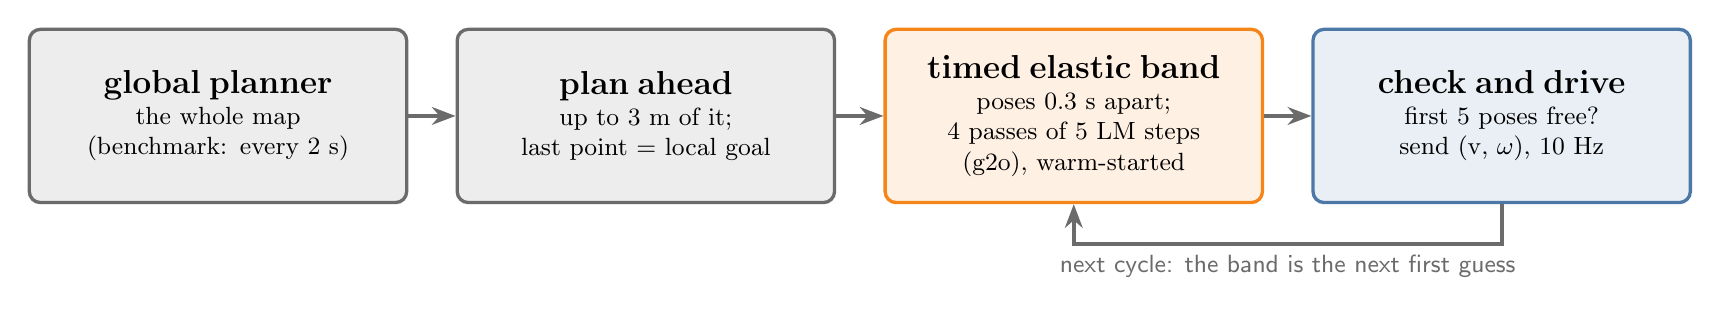
\begin{tikzpicture}[node distance=0.6cm,
  st/.style={box=#1, font=\small, minimum width=4.6cm, text width=4.3cm, minimum height=2.2cm}]
  \node[st=cgrey] (a) {{\large\textbf{global planner}}\\ the whole map\\ (benchmark: every 2 s)};
  \node[st=cgrey, right=of a] (b) {{\large\textbf{plan ahead}}\\ up to 3 m of it;\\ last point = local goal};
  \node[st=corange, right=of b] (c) {{\large\textbf{timed elastic band}}\\ poses 0.3 s apart;\\ 4 passes of 5 LM steps\\ (g2o), warm-started};
  \node[st=cblue, right=of c] (d) {{\large\textbf{check and drive}}\\ first 5 poses free?\\ send (v, $\omega$), 10 Hz};
  \draw[arrow] (a) -- (b); \draw[arrow] (b) -- (c); \draw[arrow] (c) -- (d);
  \draw[arrow] (d.south) -- ++(0,-0.5) -| node[note, pos=0.25, below] {next cycle: the band is the next first guess} (c.south);
\end{tikzpicture}
\end{document}
